This sections describes the purpose, use, and intended user audience for the Smart Hospital Management Tool. The Smart Hospital Management Tool that performs managing the inventory and keeps track of employees' schedules. The Smart Hospital faculty and students will be able to schedule simulations, check out tools, clock their worked hours, and iventory management.

\subsection{Purpose and Use}
The Smart Hospital Management Tool is a web-base software application to help the Smart Hospital manage their inventory, employee schedules, time, generated reports, and other factors. The Smart Hospital faculty and students will access the Smart Hospital Management Tool through a web browser and schedule simulations.

\subsection{Intended Audience}
The Smart Hospital Management Tool will be used by the Smart Hospital faulty, graduate students, and undergraduate students. In the future, other colleges may wish to incorporate the software which will be freely available.

\begin{figure}[h!]
	\centering
   	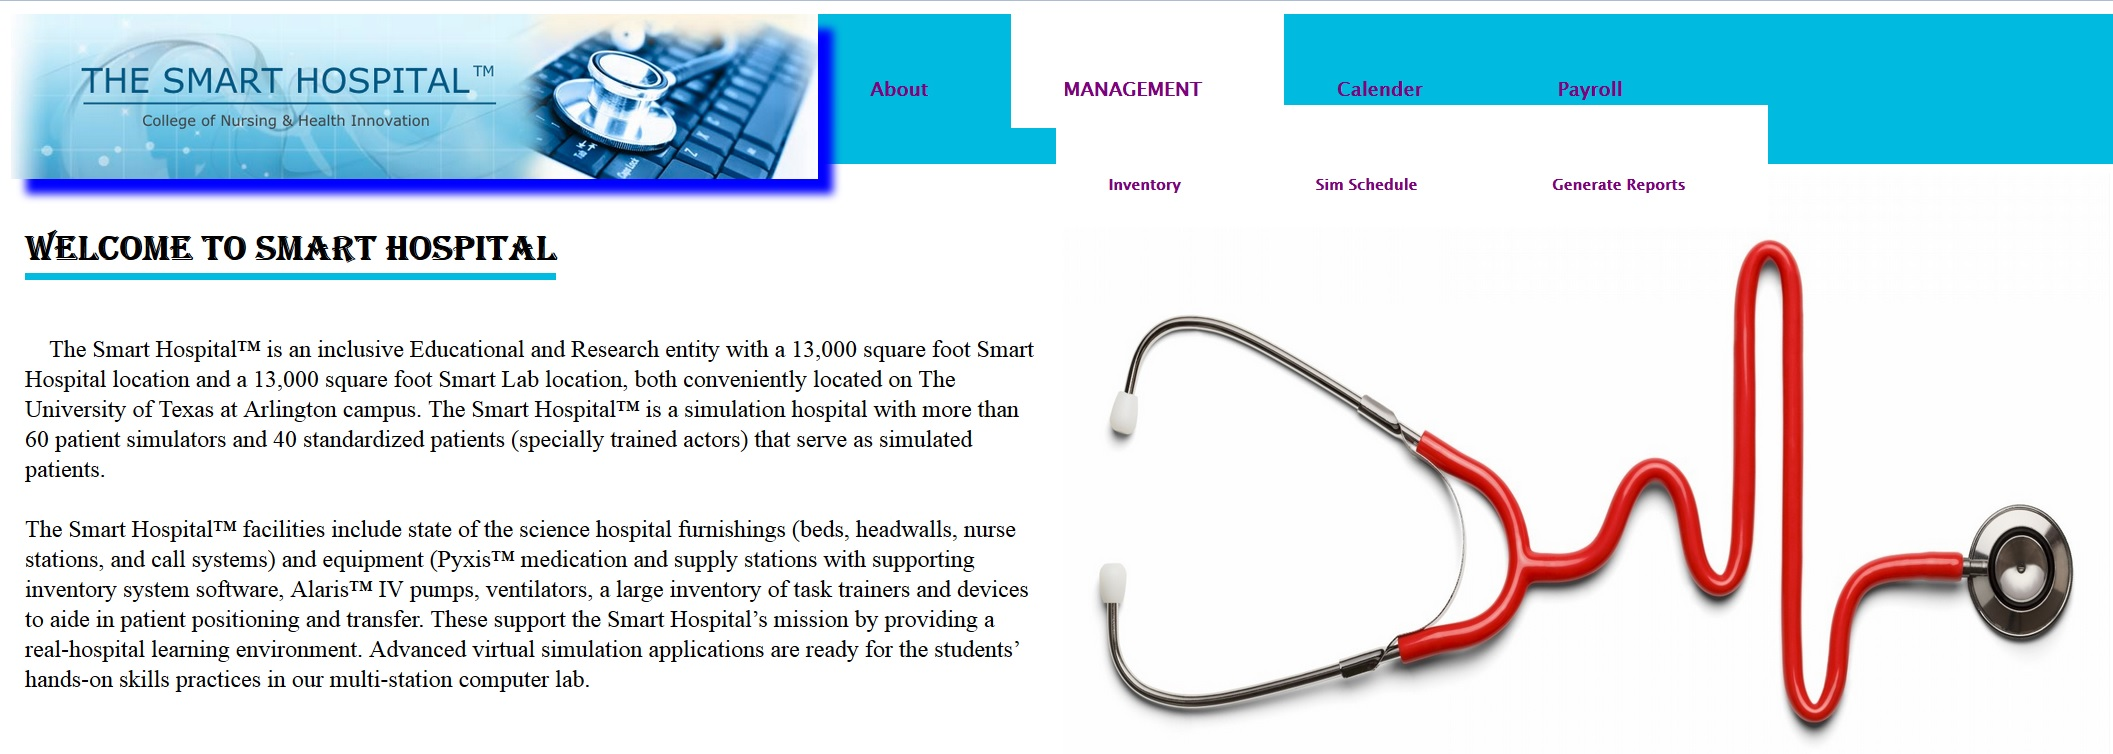
\includegraphics[width=0.60\textwidth]{images/concept_screenshot_1}
    \caption{UTASmart.com Placeholder}
\end{figure}

\begin{figure}[h!]
	\centering
   	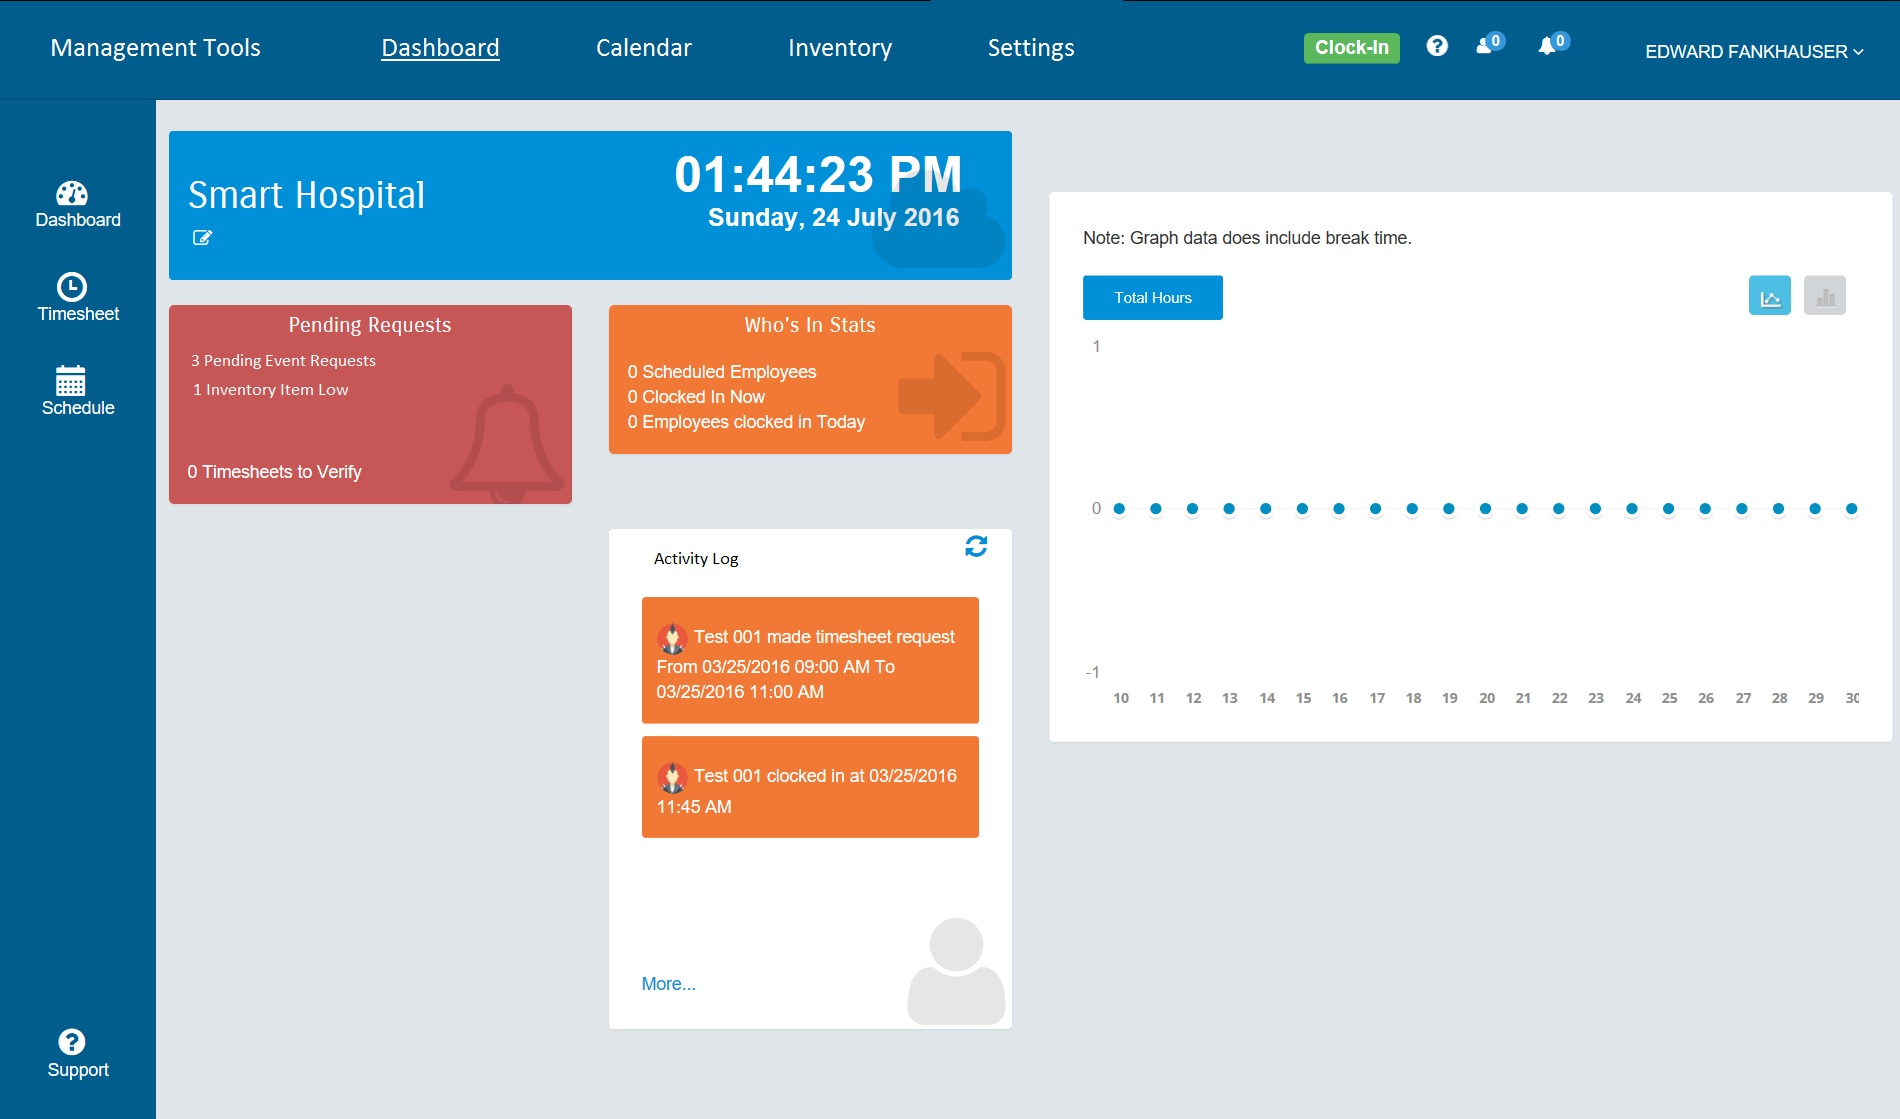
\includegraphics[width=0.60\textwidth]{images/concept_timeclock_derive}
    \caption{Timeclockwizard.com derived website}
\end{figure}
